%%%%%%%%%%%%%%%%%%%%% chapter.tex %%%%%%%%%%%%%%%%%%%%%%%%%%%%%%%%%
%
% sample chapter
%
% Use this file as a template for your own input.
%
%%%%%%%%%%%%%%%%%%%%%%%% Springer-Verlag %%%%%%%%%%%%%%%%%%%%%%%%%%
%\motto{Use the template \emph{chapter.tex} to style the various elements of your chapter content.}
\chapter{Eclipse4 Application Model}
\label{intro} % Always give a unique label
% use \chaptermark{}
% to alter or adjust the chapter heading in the running head

% command : \url \text{xx} \newline \emph 


\abstract{Eclipse4 Application 개발가이드를 정리한다.}

\section{Eclipse4 Appplication Model}
\label{sec:1}

\subsection{What is the application model?}
Eclipse4는 어플리케이션 구조를 기술하기위해 어플리케이션모델(application model)이라고 하는 추상서술\footnote{Abstract description}을 사용한다. 이러한 어플리케이션 모델은 Eclipse4 어플리케이션에 있어 비시각요소뿐만 아니라 시각요소를 포함한다. \\

예를 들어 시각적 부품으로는 윈도우(window),파츠(parts:views,editor), 메뉴(menus), 툴바(toolbars) 등이다. 비 시각요소에 대한 예를 들면 핸들러(handlers), 명령(commands), 키바인딩(key bindings)이다. \\

Fig 2.1 은 e4툴 에디터로 열어본 예제 어플리케이션 모델을 보여주고 있다. \\

\begin{figure}[hbt]
\centering
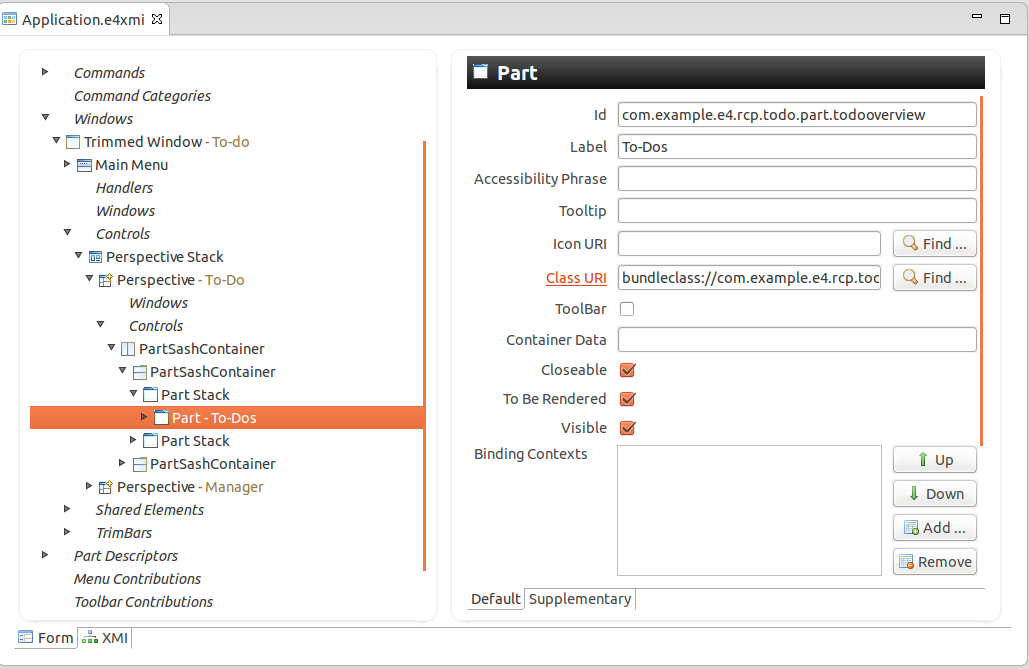
\includegraphics[scale=.32]{./image/e4_001}
\label{fig:1}       % Give a unique label
\captionsetup{justification=centering}
\caption{Application Model}
\end{figure}

각 모델 요소는 자신의 현재상태를 기술하는 속성을 가진다. 예를 크기, 위치 등이다. 대부분의 모델 요소들은 계층관계순서로 되어 있다. 에를 들어 파트는 퍼스펙티브(perspective)에 속해져 있어야 한다. \\ 

\subsection{Scope of the application model}
어플리케이션 모델은 어플리케이션 구조를 정의하지만 개별적인 사용자 인터페이스 요소의 내용을 기술하지는 않는다. \\

예를 들어, 어플리케이션 모델은 파츠의 유효함을 기술한다. 파츠의 속성 예를 들어 닫을수 있는가(cloable), 라벨, 아이디를 말한다. 그러나 각파츠들의 라벨들, 텍스트 필드및 버튼등의 내용에 대해서는 기술하지 않는다. 파츠의 내용은 여전히 소스코드에서 정의되어야 한다. \\

만약 어플리케이션 모델이 집이라면 어플리케이션 모델은 유요한 방들과 배열(perspectives, ParStacks, PartSashContainer)을 기술한다. 하지만 방에 배치되어 있는 가구들에 있어서는 기술하지 않는다. 이는 Fig 2.2로 묘사될수 있다. \\

\begin{figure}[hbt]
\centering
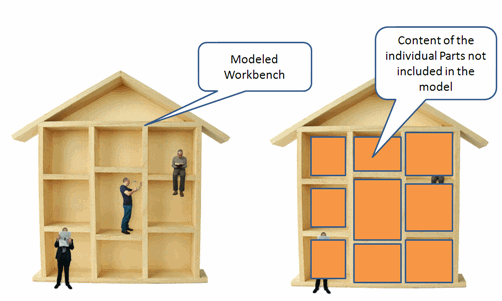
\includegraphics[scale=.50]{./image/e4_002}
\label{fig:2}       % Give a unique label
\captionsetup{justification=centering}
\caption{Application Model Depiction}
\end{figure}

\subsection{How do you define the application model?}
어플리케이션 모델의 기초는 전형적으로 정적인 파일로 정의 된다. 이 파일을 위한 기본 이름은 Application.e4xmi이고 기본 위치는 어플리케이션 플러그의 주 디렉토리가 된다. \\
%\verb|text|
\begin{svgraybox}
개발자는 \verb|org.eclipse.core.runtime.prodcuts| 확장포인터를 통해 이름과 위치를 바꿀 수 있다. \textit{applicationXMI} 파라미터의 값을 변경할 려는 어플리케이션 모델 파일의 URI로 바꾸면 된다. 이절차에 대한 상세는 ???를 살펴본다.
\end{svgraybox}

\section{User interface model elements}
\label{sec:2}대
다음의 모델요소는 개발자가 어플리케이션에서 사용자 인터페이스를 만들기 위해 사용하는 기본 요소들을 대표한다.

\subsection{Window}
이클립스 어플리케이션은 하나 또는 그이상의 윈도우로 구성된다. 전형적으로 어플리케이션은 하나의 윈도우를 가지지만 멀티모니터 지원이 필요한 경우에는 제한하지는 않는다. \\

\begin{figure}[hbt]
\centering
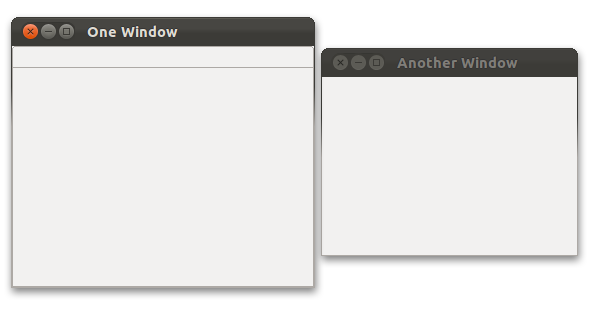
\includegraphics[scale=.50]{./image/e4_003}
\label{fig:3}       % Give a unique label
\captionsetup{justification=centering}
\caption{Multiple Window}
\end{figure}

\subsection{Views and editors-parts}
파츠(Parts)는 개발자가 네비이게트및 데이터를 정의하는 것을 허용하느  사용자 인터페이스 요소이다. 파트는 드롭다운메뉴, 컨텍스트메뉴, 툴바를 가질수 있다. \\

파츠는 사용자 인터페이스에서 자유롭게 위치할 수 있다. \\

\begin{figure}[hbt]
\centering
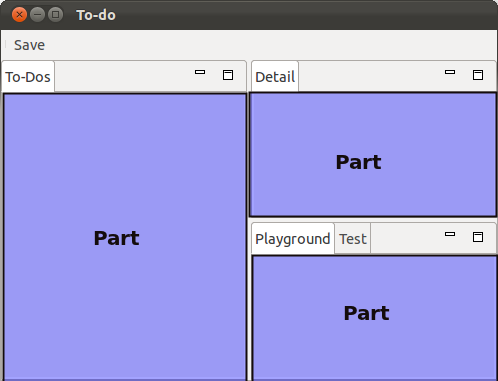
\includegraphics[scale=.50]{./image/e4_004}
\label{fig:4}       % Give a unique label
\captionsetup{justification=centering}
\caption{Parts for user interface}
\end{figure}

파츠는 전형적으로 뷰(Views)와 편집기(Editors)로 분류된다. 뷰와 데이터의 차이는 기술적 다름에 기반하지 않지만 파츠들의 사용및 배치에 다름 개념에 그 차이가 있다. \\

뷰는 전형적으로 계층적 구조로 되어 있는 데이터집합을 작업할 때 사용된다. 만일 데이터가 뮤를 통해 변경이 되면 이 변경은 해당 데이터 구조에 바로 적용된다. 뷰는 때때로 우리가 선택된 데이터를 편비하기 위한 에디터를 여는 것을 허용한다. \\

뷰를 위한 예제는 우리가 이클립스 프로젝트 파일을 검색하도록 하는 패키지 익스플러(\textit{Package Explorer})이다.만일 패키지 익스플러에서 데이터를 변경하면 파일시스템에 바로 적용된다. \\

에디터는 전형적으로 파일의 내용 또는 데이터 오브젝트 같이 하나의 데이터 요소를 수정하기 위해 사용된다. 변경내역을 적용하기 위해서는 에디터 내용을 저장해야 한다. \\

\begin{figure}[hbt]
\centering
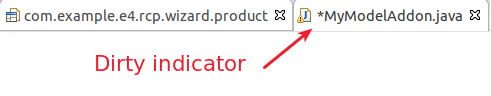
\includegraphics[scale=.50]{./image/e4_005}
\label{fig:5}       % Give a unique label
\captionsetup{justification=centering}
\caption{Editor Dirty Indicator}
\end{figure}

\subsection{Perspective}
퍼스펙티브(Perspective)는 시작요소 파츠들을 담는 컨테이너이다. 퍼스펙티브는 파츠들의 다른 배치를 저장하기 위해 사용되어 질 수 있다. 예를 들어 이클립스IDE는 개발자가 수행하기 원하는 작업(개발, 디버깅, 리뷰...)을 위한 알맞는 뷰 레이아웃을 사용한다. \\

개발자는 어플리케이션 모델의 퍼스펙티브 스택(perspective stack)에 퍼스펙티브를 놓을 수 있다. 퍼스펙티브 교환은 이클립스 플랫폼에 의해 제공되어 지는 파트 서비스를 통해 할 수 있다. \\

\subsection{PartStack and PartSashContainer}
파츠는 윈도우 또는 퍼스펙티브에 직접으로 할당될 수 있지만 개발자는 일반적으로 그것들을 그룹및 배열하고 싶어 한다. \\

이를 위해서 개발자는 \textit{PartStack} 과 \textit{PartSashContainer} 모델 요소를 사용할 수 있다. \\

파트스택(PartStack)은 모든 파츠의 헤더들을 보는 동안 어떤 파트의 내용을 보여주는 파츠집합을 포함한다. 하나의 파트는 활성화 되고 사용자는 사용자는 상응하는 탭을 선택함으로써 다른 파트로 바꿀수 있다. \\

파트컨테이너(PartSashContainer)는 수직및 수평 배열된 자식들 모두를 동시에 보여준다. \\


\begin{figure}[h]
	\centering
	\begin{subfigure}[b]{0.55\textwidth}
		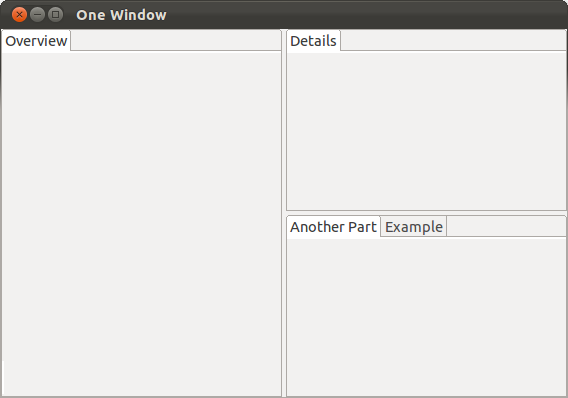
\includegraphics[width=\textwidth]{./image/e4_006}
	\end{subfigure}
	\begin{subfigure}[b]{0.4\textwidth}
		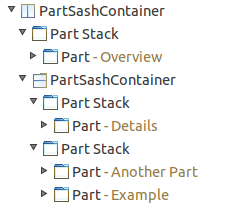
\includegraphics[width=\textwidth]{./image/e4_007}
	\end{subfigure}
	\captionsetup{justification=centering}
	\caption{PartStack and PartSashContainer}
	\label{fig:6}       % Give a unique label
\end{figure}

Figure \ref{fig:6}는 두개의 파트컨테이너와 적은 파트스택을 사용한 간단한 이클립스 어플리케이션 레이아웃을 보여준다. \\

\subsection{Using layout weight data for children elements}
레이아웃 웨이트에 할당된 파트컨테이너(PartSashContainer)의 자식 속성으로 \textit{Conainer Data}를 사용할 수 있다. \\

레이아웃 웨이트\footnote{layout weight : }는 상응하는 자식 용소가 파트컨테이너로 부터 할당되어지는 상대적인 공간으로 해독되어 진다. \\

\begin{figure}[hb]
\centering
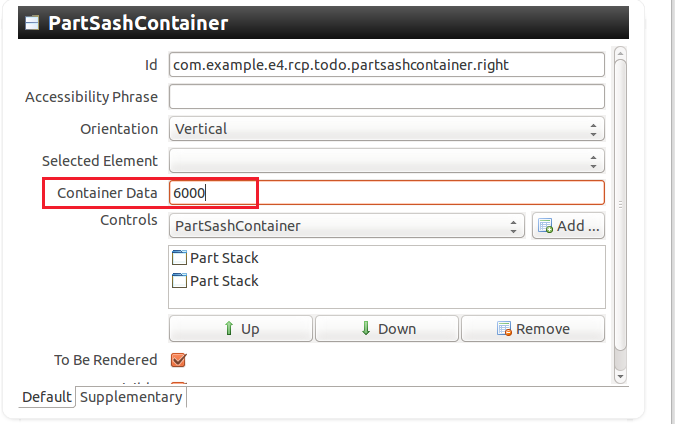
\includegraphics[scale=.50]{./image/e4_008}
\captionsetup{justification=centering}
\caption{PartSashContainer}
\label{fig:7}       % Give a unique label
\end{figure}

설정은 Figure \ref{fig:7}에 묘사되어 있다. \\

\begin{svgraybox}
	\textbf{Warnning} \\ \\
	만일 하나의 요소를 위해 \textit{Conainer Data}을 설정하면 반드시 모든 요소		에 대해서 정의 해야 한다. 달리말해 놓친 값들이 매우 높이 해독되어 지고 이러한 		요소들이 사용가능한 공간을 차지하게 된다.
\end{svgraybox}

\begin{svgraybox}
	\textbf{Tip} \\ \\
	The initial total of all the container data values is maintained 		when elements in the sash are moved. In order to allow fine 			grained/smooth dragging this total must be similar to the screen 		resolution. A too low value (i.e. 50 / 50) causes the part to be 		moved multiple pixels per sash unit, which the user will realize 		as a jerky movement. Therefore, use a sufficient high value, e.g., 	10000.
\end{svgraybox}

\section{Connecting model elements to classes and resources}

\subsection{Connect model elements to classes}
어플리케이션 모델에서 어떤 모델 요소들은 URI\footnote{Uniform Resource Identifier}를 통해 자바 클래스들 참조를 포함 할 수 있다. \\

URI는 자바 클래스의 경로를 기술한다. URI의 첫번째 파트는 플러그인이고 두번째는 패키지이고 마지막은 클래스이다. \\

\begin{figure}[h]
\centering
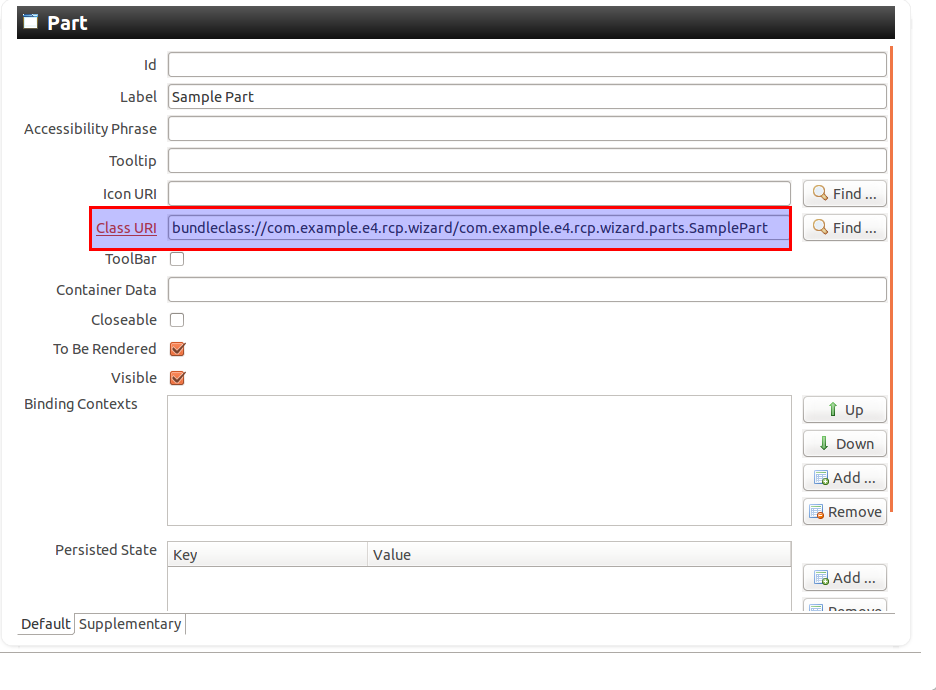
\includegraphics[scale=.35]{./image/e4_009}
\captionsetup{justification=centering}
\caption{Part}
\label{fig:9}       % Give a unique label
\end{figure}

어떤 어플리케이션 모델요소는 요소를 위한 자바 클래스을 가르키는 \textit{Class URI}속성을 가진다.이 클래스는 파트의 행위를 제공한다. 집/방 비유를 사용해서 설명하여 보면 클래스는 가구들을 정의, 가구 배치, 객체행위 상호작용을 어떻게 하는 것에 대한 책임이 있다. \\

이클립스는 참조된 클래들을 게으르게(lazily) 인스턴스화한다. 이는 클래스들이 모델요소들이 활성화 될때 인스턴ㅅ화 되는 것을 의미한다. 예를 들어 파츠들의 오브젝트들은 파트가 보이게 될때 한번 생성이 된다. \\

\subsection{Connect model elements to resources}
모델 요소들은 정적 자원들을 가르킬 수 있다. 예를 들어, 파트 모델 요소는 이클립스 플랫폼에서 파트를 나타내기 위한 \textit{icon URI} 속성을 포함한다. \\

\subsection{URI patterns}
URIs 다음의 두가지 패턴을 따른다. 하나는 \textit{classes}을 식별하기 위한 것이고 또하나는 \textit{resources}을 식별하기 위한 것이다. 다음의 테이블은 이들 두가지 패텬을 기술한다. 예는 번들은 \textit{test}라고 가정한다. \\

\begin{table}
\caption{URI Pattern}
\label{tab:1}       % Give a unique label
%
% For LaTeX tables use
%
\begin{tabular}{p{5cm}p{6.5cm}}
\hline\noalign{\smallskip}
Pattern & Description \\
\noalign{\smallskip}\svhline\noalign{\smallskip}
%row#1
bundleclass://Bundle\-SymbolicName/package.classname 
Example: \linebreak
bundleclass://test/test.parts.MySavePart & Used to identify Java classes. It consists of the following parts: "bundleclass://" is a fixed schema, Bundle\-SymbolicName as defined in the MANIFEST.MF file and separated by a '/' the fully qualified classname.  \\
\hline\noalign{\smallskip}
%row#2
platform:/plugin/Bundle\-SymbolicName/path/filename.extension 
Example: \linebreak
platform:/plugin/test/icons/save\_edit.gif & Identifier for a resource in a plug-in. "platform:/plugin/" is a fixed schema, followed by the Bundle\-SymbolicName of the MANIFEST.MF file, followed by the path to the file and the filename. \\
\noalign{\smallskip}\hline\noalign{\smallskip}
\end{tabular}
\end{table}


\subsection{Model Objects}
어플리케이션 모델 요소들의 속성은 런타임시 자바 오브젝트에 저장된다. 이 오브젝트들을 시 토튜리얼에서 모델 오브젝트라고 부른다. \\

이러한 몸델 오브젝트들은 속성들이나 하위 오브젝트들을 변경할 때 사용 할 수 있다. 이클립스 프랫폼은 모델오브젝트에 등록된 변경리스너를 가지고 있고 관련되 속성들이 변경될 때 마다 사용자인터페이스를 업데이트한다. \\

다음 테이블은 중요한 모델 오브젝트들을 목록화 한다. \\


\begin{table}
\caption{Eclipse model elements}
\label{tab:1}       % Give a unique label
%
% For LaTeX tables use
%
\begin{tabular}{p{4cm}p{7.5cm}}
\hline\noalign{\smallskip}
Model element & Description \\
\noalign{\smallskip}\svhline\noalign{\smallskip}
%row#1
MApplication & 어플리케이션 오브젝트를 기술한다. 모든 다른 모델 요소들은 이오브젝트의 아래에 있다. \\
\hline\noalign{\smallskip}
%row#2
MAddon & 사용자 인터페이스가 없는 자기충족(self-contained) 콤포넌트이다. 어플리케이션 라이프사이클에서 이벤트및 해당 이벤트의 해들러를 등록할수 있다. \\
\hline\noalign{\smallskip}
%row#3
MWindow & 어플리케이션에서 윈도우를 나타낸다. \\
\hline\noalign{\smallskip}
%row#4
MTrimmedWindow & MWindow와 비슷하지만 윈도우를 위한 툴바를 포함할 수 있다. \\
\hline\noalign{\smallskip}
%row#5
MPerspective & 퍼스펙티브 모델 요소를 위한 오브젝트. MPerspectiveStack만 포함될수 있다. \\
\hline\noalign{\smallskip}
%row#6
MPart & 모델 요소 파트를 나타낸다. \\
\hline\noalign{\smallskip}
%row#7
MDirtyable & 주입될 수 있는 MPart의 성질이다. true로 하면 이 프로퍼티는 이클립스 플랫폼에 이 파트는 저장되지 않는 데이터를 포함하고 있음을 통보한다. 핸들러 에서 저장을 트리거하기 위한 이 프로퍼티를 조회 할 수 있다. \\
\hline\noalign{\smallskip}
%row#8
MPartDescriptor & MPartDescriptor는 새로운 파츠를 위한 템플릿이다. 파트디스크립터에서 새로운 파트를 생성할 수 있고, EPartService.showPart() 함수를 통해 보여진다. \\
\hline\noalign{\smallskip}
%row#9
Snippets & 스닙펫은 프로그램을 통해 생성하기위한 미리 설정환 모델 파츠로 사용될 수 있다. 스닙펫을 복제하기위해 이클립스 EModelService를 사용하고 런타임시에 어플리케이션 모델에 스닙펫을 봍이기 우해 결과 오브젝트를 사용한다. \\
\noalign{\smallskip}\hline\noalign{\smallskip}
\end{tabular}
\end{table}

\begin{svgraybox}
	\textbf{Tip} \\ \\
	이러한 모델 오브젝트들에 접근은 어노테이션을 활용한 의존성 주입으로 행해진다.
\end{svgraybox}

\subsection{Runtime application model}



\begin{description}[Type 1]
\item[Type 1]{That addresses central themes pertainng to migration, health, and disease. In Sect.~\ref{sec:1}, Wilson discusses the role of human migration in infectious disease distributions and patterns.}
\item[Type 2]{That addresses central themes pertainng to migration, health, and disease. In Sect.~\ref{subsec:2}, Wilson discusses the role of human migration in infectious disease distributions and patterns.}
\end{description}

\subsection{Subsection Heading} %
In order to avoid simply listing headings of different levels we recommend to let every heading be followed by at least a short passage of text. Use the \LaTeX\ automatism for all your cross-references and citations citations as has already been described in Sect.~\ref{sec:2}.

Please note that the first line of text that follows a heading is not indented, whereas the first lines of all subsequent paragraphs are.

\begin{svgraybox}
If you want to emphasize complete paragraphs of texts we recommend to use the newly defined Springer class option \verb|graybox| and the newly defined environment \verb|svgraybox|. This will produce a 15 percent screened box 'behind' your text.

If you want to emphasize complete paragraphs of texts we recommend to use the newly defined Springer class option and environment \verb|svgraybox|. This will produce a 15 percent screened box 'behind' your text.
\end{svgraybox}


\subsubsection{Subsubsection Heading}
Instead of simply listing headings of different levels we recommend to let every heading be followed by at least a short passage of text. Furtheron please use the \LaTeX\ automatism for all your cross-references and citations as has already been described in Sect.~\ref{sec:2}.

Please note that the first line of text that follows a heading is not indented, whereas the first lines of all subsequent paragraphs are.

\begin{theorem}
Theorem text goes here.
\end{theorem}
%
% or
%
\begin{definition}
Definition text goes here.
\end{definition}

\begin{proof}
%\smartqed
Proof text goes here.
\qed
\end{proof}

\paragraph{Paragraph Heading} %
Instead of simply listing headings of different levels we recommend to let every heading be followed by at least a short passage of text. Furtheron please use the \LaTeX\ automatism for all your cross-references and citations as has already been described in Sect.~\ref{sec:2}.

Note that the first line of text that follows a heading is not indented, whereas the first lines of all subsequent paragraphs are.
%
% For built-in environments use
%
\begin{theorem}
Theorem text goes here.
\end{theorem}
%
\begin{definition}
Definition text goes here.
\end{definition}
%
\begin{proof}
\smartqed
Proof text goes here.
\qed
\end{proof}
%
\begin{acknowledgement}
If you want to include acknowledgments of assistance and the like at the end of an individual chapter please use the \verb|acknowledgement| environment -- it will automatically render Springer's preferred layout.
\end{acknowledgement}
%
\section*{Appendix}
\addcontentsline{toc}{section}{Appendix}
%
When placed at the end of a chapter or contribution (as opposed to at the end of the book), the numbering of tables, figures, and equations in the appendix section continues on from that in the main text. Hence please \textit{do not} use the \verb|appendix| command when writing an appendix at the end of your chapter or contribution. If there is only one the appendix is designated ``Appendix'', or ``Appendix 1'', or ``Appendix 2'', etc. if there is more than one.

\begin{equation}
a \times b = c
\end{equation}
% Problems or Exercises should be sorted chapterwise
\section*{Problems}
\addcontentsline{toc}{section}{Problems}
%
% Use the following environment.
% Don't forget to label each problem;
% the label is needed for the solutions' environment
\begin{prob}
\label{prob1}
A given problem or Excercise is described here. The
problem is described here. The problem is described here.
\end{prob}

\begin{prob}
\label{prob2}
\textbf{Problem Heading}\\
(a) The first part of the problem is described here.\\
(b) The second part of the problem is described here.
\end{prob}

%%%%%%%%%%%%%%%%%%%%%%%% referenc.tex %%%%%%%%%%%%%%%%%%%%%%%%%%%%%%
% sample references
% %
% Use this file as a template for your own input.
%
%%%%%%%%%%%%%%%%%%%%%%%% Springer-Verlag %%%%%%%%%%%%%%%%%%%%%%%%%%
%
% BibTeX users please use
% \bibliographystyle{}
% \bibliography{}
%
\biblstarthook{In view of the parallel print and (chapter-wise) online publication of your book at \url{www.springerlink.com} it has been decided that -- as a genreral rule --  references should be sorted chapter-wise and placed at the end of the individual chapters. However, upon agreement with your contact at Springer you may list your references in a single seperate chapter at the end of your book. Deactivate the class option \texttt{sectrefs} and the \texttt{thebibliography} environment will be put out as a chapter of its own.\\\indent
References may be \textit{cited} in the text either by number (preferred) or by author/year.\footnote{Make sure that all references from the list are cited in the text. Those not cited should be moved to a separate \textit{Further Reading} section or chapter.} The reference list should ideally be \textit{sorted} in alphabetical order -- even if reference numbers are used for the their citation in the text. If there are several works by the same author, the following order should be used: 
\begin{enumerate}
\item all works by the author alone, ordered chronologically by year of publication
\item all works by the author with a coauthor, ordered alphabetically by coauthor
\item all works by the author with several coauthors, ordered chronologically by year of publication.
\end{enumerate}
The \textit{styling} of references\footnote{Always use the standard abbreviation of a journal's name according to the ISSN \textit{List of Title Word Abbreviations}, see \url{http://www.issn.org/en/node/344}} depends on the subject of your book:
\begin{itemize}
\item The \textit{two} recommended styles for references in books on \textit{mathematical, physical, statistical and computer sciences} are depicted in ~\cite{science-contrib, science-online, science-mono, science-journal, science-DOI} and ~\cite{phys-online, phys-mono, phys-journal, phys-DOI, phys-contrib}.
\item Examples of the most commonly used reference style in books on \textit{Psychology, Social Sciences} are~\cite{psysoc-mono, psysoc-online,psysoc-journal, psysoc-contrib, psysoc-DOI}.
\item Examples for references in books on \textit{Humanities, Linguistics, Philosophy} are~\cite{humlinphil-journal, humlinphil-contrib, humlinphil-mono, humlinphil-online, humlinphil-DOI}.
\item Examples of the basic Springer style used in publications on a wide range of subjects such as \textit{Computer Science, Economics, Engineering, Geosciences, Life Sciences, Medicine, Biomedicine} are ~\cite{basic-contrib, basic-online, basic-journal, basic-DOI, basic-mono}. 
\end{itemize}
}

\begin{thebibliography}{99.}%
% and use \bibitem to create references.
%
% Use the following syntax and markup for your references if 
% the subject of your book is from the field 
% "Mathematics, Physics, Statistics, Computer Science"
%
% Contribution 
\bibitem{science-contrib} Broy, M.: Software engineering --- from auxiliary to key technologies. In: Broy, M., Dener, E. (eds.) Software Pioneers, pp. 10-13. Springer, Heidelberg (2002)
%
% Online Document
\bibitem{science-online} Dod, J.: Effective substances. In: The Dictionary of Substances and Their Effects. Royal Society of Chemistry (1999) Available via DIALOG. \\
\url{http://www.rsc.org/dose/title of subordinate document. Cited 15 Jan 1999}
%
% Monograph
\bibitem{science-mono} Geddes, K.O., Czapor, S.R., Labahn, G.: Algorithms for Computer Algebra. Kluwer, Boston (1992) 
%
% Journal article
\bibitem{science-journal} Hamburger, C.: Quasimonotonicity, regularity and duality for nonlinear systems of partial differential equations. Ann. Mat. Pura. Appl. \textbf{169}, 321--354 (1995)
%
% Journal article by DOI
\bibitem{science-DOI} Slifka, M.K., Whitton, J.L.: Clinical implications of dysregulated cytokine production. J. Mol. Med. (2000) doi: 10.1007/s001090000086 
%
\bigskip

% Use the following (APS) syntax and markup for your references if 
% the subject of your book is from the field 
% "Mathematics, Physics, Statistics, Computer Science"
%
% Online Document
\bibitem{phys-online} J. Dod, in \textit{The Dictionary of Substances and Their Effects}, Royal Society of Chemistry. (Available via DIALOG, 1999), 
\url{http://www.rsc.org/dose/title of subordinate document. Cited 15 Jan 1999}
%
% Monograph
\bibitem{phys-mono} H. Ibach, H. L\"uth, \textit{Solid-State Physics}, 2nd edn. (Springer, New York, 1996), pp. 45-56 
%
% Journal article
\bibitem{phys-journal} S. Preuss, A. Demchuk Jr., M. Stuke, Appl. Phys. A \textbf{61}
%
% Journal article by DOI
\bibitem{phys-DOI} M.K. Slifka, J.L. Whitton, J. Mol. Med., doi: 10.1007/s001090000086
%
% Contribution 
\bibitem{phys-contrib} S.E. Smith, in \textit{Neuromuscular Junction}, ed. by E. Zaimis. Handbook of Experimental Pharmacology, vol 42 (Springer, Heidelberg, 1976), p. 593
%
\bigskip
%
% Use the following syntax and markup for your references if 
% the subject of your book is from the field 
% "Psychology, Social Sciences"
%
%
% Monograph
\bibitem{psysoc-mono} Calfee, R.~C., \& Valencia, R.~R. (1991). \textit{APA guide to preparing manuscripts for journal publication.} Washington, DC: American Psychological Association.
%
% Online Document
\bibitem{psysoc-online} Dod, J. (1999). Effective substances. In: The dictionary of substances and their effects. Royal Society of Chemistry. Available via DIALOG. \\
\url{http://www.rsc.org/dose/Effective substances.} Cited 15 Jan 1999.
%
% Journal article
\bibitem{psysoc-journal} Harris, M., Karper, E., Stacks, G., Hoffman, D., DeNiro, R., Cruz, P., et al. (2001). Writing labs and the Hollywood connection. \textit{J Film} Writing, 44(3), 213--245.
%
% Contribution 
\bibitem{psysoc-contrib} O'Neil, J.~M., \& Egan, J. (1992). Men's and women's gender role journeys: Metaphor for healing, transition, and transformation. In B.~R. Wainrig (Ed.), \textit{Gender issues across the life cycle} (pp. 107--123). New York: Springer.
%
% Journal article by DOI
\bibitem{psysoc-DOI}Kreger, M., Brindis, C.D., Manuel, D.M., Sassoubre, L. (2007). Lessons learned in systems change initiatives: benchmarks and indicators. \textit{American Journal of Community Psychology}, doi: 10.1007/s10464-007-9108-14.
%
%
% Use the following syntax and markup for your references if 
% the subject of your book is from the field 
% "Humanities, Linguistics, Philosophy"
%
\bigskip
%
% Journal article
\bibitem{humlinphil-journal} Alber John, Daniel C. O'Connell, and Sabine Kowal. 2002. Personal perspective in TV interviews. \textit{Pragmatics} 12:257--271
%
% Contribution 
\bibitem{humlinphil-contrib} Cameron, Deborah. 1997. Theoretical debates in feminist linguistics: Questions of sex and gender. In \textit{Gender and discourse}, ed. Ruth Wodak, 99--119. London: Sage Publications.
%
% Monograph
\bibitem{humlinphil-mono} Cameron, Deborah. 1985. \textit{Feminism and linguistic theory.} New York: St. Martin's Press.
%
% Online Document
\bibitem{humlinphil-online} Dod, Jake. 1999. Effective substances. In: The dictionary of substances and their effects. Royal Society of Chemistry. Available via DIALOG. \\
http://www.rsc.org/dose/title of subordinate document. Cited 15 Jan 1999
%
% Journal article by DOI
\bibitem{humlinphil-DOI} Suleiman, Camelia, Daniel C. O Connell, and Sabine Kowal. 2002. `If you and I, if we, in this later day, lose that sacred fire...': Perspective in political interviews. \textit{Journal of Psycholinguistic Research}. doi: 10.1023/A:1015592129296.
%
%
%
\bigskip
%
%
% Use the following syntax and markup for your references if 
% the subject of your book is from the field 
% "Computer Science, Economics, Engineering, Geosciences, Life Sciences"
%
%
% Contribution 
\bibitem{basic-contrib} Brown B, Aaron M (2001) The politics of nature. In: Smith J (ed) The rise of modern genomics, 3rd edn. Wiley, New York 
%
% Online Document
\bibitem{basic-online} Dod J (1999) Effective Substances. In: The dictionary of substances and their effects. Royal Society of Chemistry. Available via DIALOG. \\
\url{http://www.rsc.org/dose/title of subordinate document. Cited 15 Jan 1999}
%
% Journal article by DOI
\bibitem{basic-DOI} Slifka MK, Whitton JL (2000) Clinical implications of dysregulated cytokine production. J Mol Med, doi: 10.1007/s001090000086
%
% Journal article
\bibitem{basic-journal} Smith J, Jones M Jr, Houghton L et al (1999) Future of health insurance. N Engl J Med 965:325--329
%
% Monograph
\bibitem{basic-mono} South J, Blass B (2001) The future of modern genomics. Blackwell, London 
%
\end{thebibliography}

